% Generated by reproduction/framework_experiments/build_manuscript_assets.py.
\subsection{三个问题的数值证据}
\label{num:scope}
实验对应推导中的三个问题：P1 核查矩阵实现及其所声明的几何结构；P2 检验通过物理磁端口实现的残差补偿；P3 区分向实际闭环向量场的收敛与标称目标的恢复。所有磁模型计算均采用重新核实来源后的梁与末端磁芯基准。合成矩阵核查另行声明其无量纲参数。参考跟踪扩展保留在补充材料第~\ref{num:route-b}~节，并使用其自身的目标和评价协议。

物理输入不确定性、空间与模态近似、系数辨识、时间积分和反馈误差属于不同的误差来源。网格收敛不能衡量两模态截断误差；很小的积分拟合残差不能给出解析范数的上界；很小的轨迹误差也不能构成不变环面证书。下列实验为各个接口分别设置数值核查问题。

\subsection{P1：矩阵实现、阶数与结构}
\label{num:p1}
对 $n=1,2,4$，取
\begin{equation}
 \begin{split}
 M&=\operatorname{diag}(1+j/5)_{j=0}^{n-1}
       +0.12\boldsymbol1\boldsymbol1^{\mathsf T},\\
 K&=\operatorname{diag}(1+j)_{j=0}^{n-1}
       +0.05\boldsymbol1\boldsymbol1^{\mathsf T},\qquad C=0.2M.
 \end{split}
 \label{num:matrix-data}
\end{equation}
这些矩阵是人工验证基准，并非导管材料参数。每个维数均采用固定初态、$T=4$ 和步长 $0.08,0.04,0.02,0.01$。在最细公共时间网格的每一点独立计算矩阵指数。误差取全部保存时刻上的最大欧氏状态误差，而非仅取终点误差。对 $n=2,4$，$M$ 与 $K$ 不可交换。

完整普通中点方程与保持正确乘法次序的消元更新在整条轨迹上相符，最大差异为 $5.3959\times10^{-15}$。另一组代数核查采用 $C_g=0.2M+0.03vv^{\mathsf T}/(v^{\mathsf T}v)$，$v=(1,\ldots,n)^{\mathsf T}$。它进一步检验 $C_gM^{-1}$ 的乘法次序：对于 $C_g$，当 $n=2,4$ 时为非比例阻尼；当 $n=1$ 时，它必然只是标量对照。该组的最大轨迹差异为 $4.6926\times10^{-15}$。不对这组附加模型声称存在共同的指数加权结构。

\begin{table*}[t]
\centering
\caption{P1 矩阵验证。观测阶由最后一次步长减半的全网格最大误差计算。保守列采用刚度为 $K+K_s$、$K_s=0.05\operatorname{diag}(1,\ldots,n)$ 的二次目标。}
\label{num:matrix-benchmark}
\small
\begin{tabular}{rccccc}
\toprule
$n$ & 最大消元差异 & 普通中点 & 加权中点 & 保守中点 & 保守 Central4\\
\midrule
1 & $1.144\times10^{-15}$ & $1.999964$ & $1.999942$ & $1.999944$ & $3.999945$ \\
2 & $4.767\times10^{-15}$ & $1.999935$ & $1.999876$ & $1.999890$ & $3.999813$ \\
4 & $5.396\times10^{-15}$ & $1.999869$ & $1.999821$ & $1.999823$ & $3.999864$ \\
\bottomrule
\end{tabular}
\end{table*}

含阻尼的普通中点法与加权 Birkhoff 中点法均呈二阶收敛，但其几何诊断不同。在 $n=2$、$\Delta=0.08$ 时，普通映射的指数加权缺陷为 $3.9280\times10^{-5}$，加权映射的缺陷为 $1.1631\times10^{-16}$。这里的缺陷定义为 $\|D\Psi^{\mathsf T}JD\Psi-e^{-0.2\Delta}J\|_2$。对于保守二次目标，中点法与 Central4 的标准辛缺陷均处于舍入误差量级，收敛阶分别为二阶和四阶。整形输入已完整指定；不能据此将四阶结论赋予任意含阻尼的反馈更新。

在新的物理坐标下，完整非线性磁势也接受同样的结构区分核查。对于未补偿的合成受控对象，普通中点法和加权中点法的最终观测阶分别为 $1.999452$ 和 $1.999400$，积分区间为 $0\leq\tau\leq4$。在 $\Delta=0.04$ 时，普通映射的指数加权缺陷为 $2.8763\times10^{-5}$；全部测试步长中，加权映射的最大缺陷为 $4.4412\times10^{-16}$。对应的已知误差闭环向量场对照也呈现相同的结构区别。这些实验在求得的数值点上评价隐式理想切映射，既不证明浮点 Newton 程序具有严格辛性，也不让学习控制器读取未知误差。

\begin{figure*}[t]
\centering
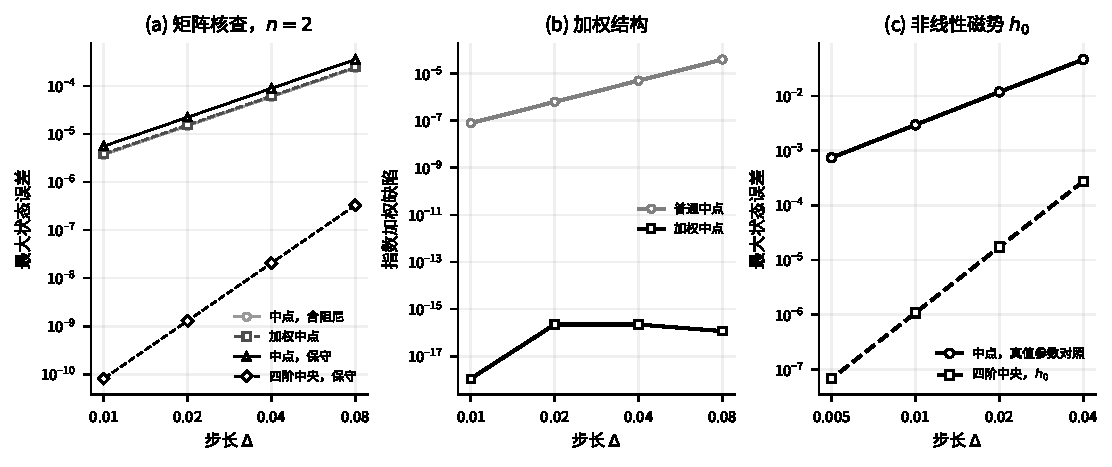
\includegraphics[width=\textwidth]{figures/framework_matrix_checks.pdf}
\caption{P1 的映射实现核查。(a) $n=2$ 时相对独立矩阵指数的全网格误差；含阻尼组与保守组分别采用各自声明的精确目标。(b) 普通与加权含阻尼中点法的指数加权缺陷。(c) 中点法与 Central4 作用于同一非线性保守磁模型 $h_0$；这些曲线比较的是同一个哈密顿量的不同离散方法。全部坐标、矩阵、初态及参考设置均记录在 JSON 中。}
\label{num:matrix-structure}
\end{figure*}

\subsection{共同物理基准与模态坐标}
\label{num:fe}
基准采用配套的材料参考值 $E\simeq2.1$ MPa 与 $\rho\simeq1028$ kg/m$^3$，并遵循 \citet{cho2021pdms} 所述的制备条件。自由长度 $80$ mm 和半径 $0.6$ mm 是研究设计输入。标称边长 $0.250$ mm 的立方磁芯采用 $B_r=1.425$ T 和密度 $7500$ kg/m$^3$，并保留其制造商牌号规格与标称选值的来源性质 \citep{smN50,kjMoment}。磁芯平动质量与转动惯量在降阶前计入有限元质量矩阵。将一致质量离散下 $16/32/64$ 个单元的频率与独立连续体边界方程根比较。前四阶模态的最大相对误差分别为 $9.59029\times10^{-6}$（$32$ 个单元）和 $6.02081\times10^{-7}$（$64$ 个单元）（表~\ref{sx:fe-table}）。

采用的 $32$ 单元坐标为
\begin{align}
 \omega_0=\omega_1&=7.84000916\ \mathrm{rad/s},\notag\\
 \omega_2&=47.39957662\ \mathrm{rad/s},\qquad
 \nu_2=6.04585730,\notag\\
 d&=\bigl(0.30722439,\,0.45042632\bigr)^{\mathsf T},\notag\\
 \ell&=\bigl(0.0189673443,\,0.0077534761\bigr)^{\mathsf T}\ \mathrm m.
 \label{num:scales}
\end{align}
生成函数、控制器和物理读出均采用相同映射。所声明基准 $C=\alpha M_{\mathrm{total}}$ 的参数为 $\zeta_1^{\mathrm d}=0.025$、$\alpha=0.3920004581$ s$^{-1}$ 和 $\gamma=0.05$，由此得到 $\zeta_2^{\mathrm d}=0.0041350629$。这些阻尼比是设计选择，并非所声明梁的实测损耗。材料、惯量及剩磁的敏感性点另见表~\ref{sx:sensitivity-table}；它们不是置信区间，也不构成高模态控制验证。

\subsection{P2：通过磁端口实现学习残差补偿}
\label{num:p2}
\label{num:route-a}
相对 $h_0$ 的受控合成偏差由一个势能特征给出。定义
\begin{equation}
 \begin{split}
 \phi(X)&=\nabla_X g(d^{\mathsf T}X)\\
        &=d[\sin(d^{\mathsf T}X)-d^{\mathsf T}X],
 \end{split}
 \label{num:feature-gradient}
\end{equation}
以及
\begin{equation}
 \begin{split}
 R_*(X)&=\beta_*g(d^{\mathsf T}X),\qquad \beta_*=0.2,\\
 \widehat R(X)&=\widehat\beta g(d^{\mathsf T}X).
 \end{split}
 \label{num:feature}
\end{equation}
系数 $0.2$ 是明确声明的压力测试设置，并非辨识得到的材料偏差。加上阻尼系数后，待拟合量只有两个标量。恢复这两个系数并不衡量完整 CHNN 优化，也不衡量对更丰富残差族的泛化。

\label{num:identification}
四条训练轨迹和两条独立验证轨迹各持续 $\tau=4$。每隔 $0.002$ 观测一次无噪声状态，采用长度为 $0.04$ 的 Simpson 积分窗，得到 $400$ 个训练向量增量，即 $800$ 个标量行。对于 $W=[\tau_a,\tau_b]$，积分平衡为
\begin{equation}
 \begin{split}
 b_W&=Y_b-Y_a+\int_W\{\mathsf NX+\phi(X)\}\,\mathrm d\tau,\\
 A_W&=\left[-\int_W\phi(X)\,\mathrm d\tau,
                 -\int_WY\,\mathrm d\tau\right],\\
 A_W\binom{\beta}{\gamma}&\simeq b_W.
 \end{split}
 \label{num:regression}
\end{equation}
经列缩放的无约束最小二乘给出
\begin{equation}
 \widehat\beta=0.200003368491,\qquad
 \widehat\gamma=0.04999999998680.
 \label{num:fitted-values}
\end{equation}
训练与留出验证的增量 RMS 残差分别为 $1.0123\times10^{-12}$ 和 $9.2492\times10^{-13}$。原始与缩放后设计矩阵的条件数分别为 $10418.25$ 和 $1.04537179$。归一化 Gram 矩阵满足 $\lambda_{\min}(G)=5.15486\times10^{-14}$，因此即使缩放后的求解条件良好，弱特征激励仍然重要。依赖真值计算的系数误差 $3.36849\times10^{-6}$ 是合成诊断量；第~\ref{sec:kam}~节的解析估计仍需要独立论证的积分与观测缺陷上界。

四个恢复组均从 $(0.09,0.08,0.015,-0.01)$ 出发，积分至 $\tau=20$（$2.551017$ s），中点步长为 $0.001$。每个非零指令都在积分过程中转换为物理磁力／磁力矩及场／梯度，经重构后代回受控对象。只有明确标出的真值参数对照使用真实系数。各组均与从相同初态独立积分得到的 $h_0$ 轨迹比较。

\begin{table*}[t]
\centering
\caption{P2 通过同一物理端口映射恢复目标。状态与末端 RMS 采用独立的 $h_0$ RK4 参考；能量变化为无量纲标称量 $\max_k|h_0(x_k)-h_0(x_0)|$。}
\label{num:a-table}
\begin{tabular}{lccc}
\toprule
控制 & 状态 RMS & 末端 RMS ($\mu$m) & 最大标称能量变化\\
\midrule
无控制 & $2.92453\times10^{-2}$ & $322.376137$ & $1.50142\times10^{-2}$ \\
阻尼补偿 & $2.43437\times10^{-5}$ & $0.143531$ & $1.37056\times10^{-7}$ \\
学习恢复 & $1.71438\times10^{-5}$ & $0.094120$ & $5.64520\times10^{-12}$ \\
真值参数恢复 & $1.71439\times10^{-5}$ & $0.094120$ & $3.24493\times10^{-12}$ \\
\bottomrule
\end{tabular}
\end{table*}

在该理想两模态实验中，拟合得到的恢复控制将状态 RMS 降至 $1.71438\times10^{-5}$，末端 RMS 降至 $0.094120\,\mu$m。其采样连续向量场失配 RMS 为 $2.5942\times10^{-11}$，但轨迹误差仍接近真值参数对照的 $1.71439\times10^{-5}$，因为二者包含相同的中点相位误差。学习组略小的误差可以由两种小误差相互抵消产生，不能作为优于真实参数控制的证据。这里检验的是从共同初态恢复目标轨迹，而非从跟踪偏移出发的吸引性。

\subsection{P3：向实际受控动力学的收敛}
\label{num:p3}
\label{num:integration}
保留主要的非线性真值参数中点对照。以 $0.04,0.02,0.01,0.005$ 逐次减半步长，最终观测阶为 $1.999331$，比较基准为独立 RK4 参考；该参考的步长加密差异为 $6.3600\times10^{-12}$。新增 Central4 实验采用同一个完整余弦保守 $h_0$，其全部导数见补充材料式~\eqref{ss:central4-magnetic-jacobian}；该方法并非在无关映射之后追加控制跳变。最终观测阶为 $3.999503$。独立 DOP853 参考加密差异为 $1.1642\times10^{-11}$，低于所报告的最小 Central4 误差。解析增量 Jacobian 在指定核查状态处与复步长微分的最大差异为 $2.7756\times10^{-17}$。

\begin{table*}[t]
\centering
\caption{非线性保守 $h_0$ 积分至 $\tau=20$。误差取全部保存时刻相对独立参考的最大值。中点法对应已有的完全补偿实验；Central4 对应新增保守格式核查。}
\label{num:nonlinear-order}
\begin{tabular}{rcccc}
\toprule
$\Delta$ & 中点误差 & 中点观测阶 & Central4 误差 & Central4 观测阶\\
\midrule
$0.04$ & $4.64310\times10^{-2}$ & --- & $2.75432\times10^{-4}$ & --- \\
$0.02$ & $1.18409\times10^{-2}$ & $1.971306$ & $1.73275\times10^{-5}$ & $3.990559$ \\
$0.01$ & $2.96760\times10^{-3}$ & $1.996414$ & $1.08474\times10^{-6}$ & $3.997648$ \\
$0.005$ & $7.42245\times10^{-4}$ & $1.999331$ & $6.78193\times10^{-8}$ & $3.999503$ \\
\bottomrule
\end{tabular}
\end{table*}

为区分数值收敛与模型恢复，另设实验固定非零辨识误差 $\delta\beta=0.02$、$\delta\gamma=0.01$。因此，同一声明受控对象上的控制器采用 $\widehat\beta=0.18$、$\widehat\gamma=0.04$。这些是人为设置的测试误差，并非前述拟合的输出或实测不确定性。实际向量场为
\begin{equation}
 \begin{split}
 X'&=\mathsf NY,\\
 Y'&=-\mathsf NX-(1+0.02)\phi(X)-0.01Y.
 \end{split}
 \label{num:fixed-error-field}
\end{equation}
中点闭环仍使用物理指令重构。独立的 DOP853 实现直接积分上述显式约化向量场；两种实现的采样向量场差异至多为 $1.1189\times10^{-16}$。所有步长均保持同一组控制系数不变。

\begin{table*}[t]
\centering
\caption{P3 的固定非零辨识误差实验。第一种误差相对同一实际连续闭环向量场计算；末列误差相对标称 $h_0$ 计算。二者均为全网格最大欧氏误差。}
\label{num:closed-convergence}
\begin{tabular}{rccc}
\toprule
$\Delta$ & 相对实际闭环的误差 & 观测阶 & 相对标称 $h_0$ 的误差\\
\midrule
$0.04$ & $4.20319\times10^{-2}$ & --- & $4.56736\times10^{-2}$ \\
$0.02$ & $1.07152\times10^{-2}$ & $1.971829$ & $1.60584\times10^{-2}$ \\
$0.01$ & $2.68521\times10^{-3}$ & $1.996545$ & $1.17602\times10^{-2}$ \\
$0.005$ & $6.71600\times10^{-4}$ & $1.999364$ & $1.14312\times10^{-2}$ \\
$0.0025$ & $1.67917\times10^{-4}$ & $1.999855$ & $1.14090\times10^{-2}$ \\
\bottomrule
\end{tabular}
\end{table*}

相对实际向量场的误差降至 $1.67917\times10^{-4}$，最终观测阶为 $1.999855$，而相对标称目标的误差趋于 $1.14090\times10^{-2}$。独立积分这两个连续模型，在最细公共网格上得到的最大差异为 $1.14070\times10^{-2}$。因此，减小步长能分辨实际闭环动力学，但不能消除所设置的建模误差。独立参考的加密差异为 $1.0636\times10^{-11}$。这一结果直接说明了收敛估计式~\eqref{ctrl:global-error} 的作用范围。

\label{num:defect-budget}
另用独立的单自由度谐振子诊断检验代数残差项。在二维相空间中，对中点增量方程人为加入 $r_k=0.01\Delta^q(1,0)^{\mathsf T}$、$q=1,2,3$，在 $T=4$ 上求解扰动后的方程。逐步保存原方程的每个实际残差。这是人为构造的代数缺陷，并非实测 Newton 停止误差，也不是导管实验。相对未扰动中点轨迹，新增误差的最终观测阶为 $0.000000,\,1.000000,\,2.000000$；它与 $\eta_\Delta/\Delta$ 的比值约为 $1.999999$。相对连续振子的总误差最终观测阶依次为 $0.000566,\,1.018776,\,1.999969$。其中 $q=3$ 保持二阶，而 $q=1$ 留下不消失的误差。该实验核查误差预算的缩放规律，并不确定定理常数的普适锐值。

\begin{figure*}[t]
\centering
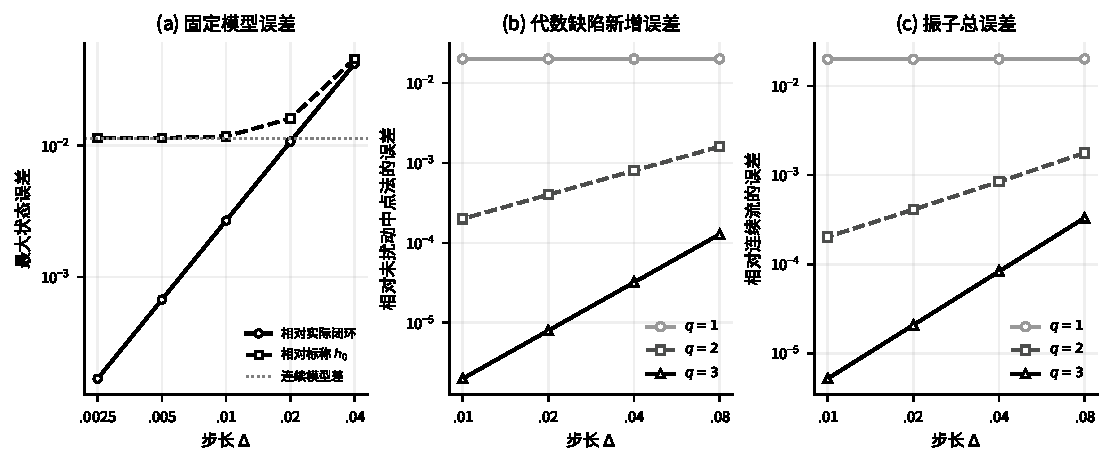
\includegraphics[width=\textwidth]{figures/framework_closed_loop_checks.pdf}
\caption{P3 区分数值误差与模型误差。(a) 固定 $\delta\beta=0.02$、$\delta\gamma=0.01$ 时，中点法收敛至实际闭环向量场，而其相对 $h_0$ 的误差趋于连续模型之差。(b) 人为增量缺陷引起的新增误差，以未扰动中点法为比较基准。(c) 相对独立连续振子的总误差；只有这项诊断采用独立的单自由度测试模型。}
\label{num:closed-results}
\end{figure*}

\subsection{阻尼情景、采样域与适用边界}
\label{num:damping}
对附加阻尼比 $\zeta_1^{\mathrm d}\in\{0,0.01,0.025,0.05,0.1\}$，分别重新生成训练／验证轨迹并重新拟合。恢复实验采用 $\tau\in[0,10]$、中点步长 $0.002$ 和独立 RK4 参考。表~\ref{sx:framework-damping-a} 给出无控制、学习及真值参数对照结果。这是模型族内的敏感性研究，并非检验一个冻结控制器抵抗未知阻尼变化。实际估计器明确采用无约束求解，并未隐式实现非负约束拟合。在真实阻尼为零时，它返回 $\widehat\gamma=-1.4038\times10^{-12}$；不将这一数值解释为材料具有负损耗。材料损耗依赖制备条件和频率，若无额外模型或器件测量，不能据此辨识这些模态阻尼比 \citep{fischer2017adhesion}。

\label{num:ports}
磁端口矩阵经列归一化后的条件数为 $3.8185963$；由于各列量纲不同，原始条件数不能被解释为与单位无关的指标。主要学习恢复实验的需求为 $\max|B_y|=0.544490$ mT 和 $\max\|\nabla B\|_2=0.01603429$ T/m。计入纵向偏置场后，最大局部磁场为 $30.004941$ mT。已发表磁系统可以提供场强量级的对照 \citep{lussi2021cvs}，但不能证明这些指令的联合场／梯度可实现性或带宽。采样末端角度与整梁斜率保持在所声明的小斜率诊断域内；这里没有认证连续时间或空间上的极值。

实验未执行饱和或输入功约束器。对于净 $4$ mm 间隙，$E_c=10.019717$ nJ，$0.95E_c=9.518731$ nJ，而主要实验的初始标称能量为 $12.656721$ nJ。因此，初始化时尚不满足所提出的充分能量上限前提。这些框架实验验证了矩阵一致性、特定收敛阶、代数磁端口实现及所述收敛区分。完整网络拟合、高模态受迫轨迹、COMSOL 对比、长时间频率研究和有限域 KAM 证书仍需单独完成。补充材料第~\ref{sx:migration}~节保留了这些早期结果的状态。
